\runningheader{SAT Mathematics}{Drill Set 6}{Page \thepage\ of \numpages}

\begingradingrange{sat-drill-06}
\subsection*{SAT Drill 6}

\question[1]
Circle A in the $xy$-plane has the equation $(x+5)^2+(y-5)^2=4$. Circle B has the same center as circle A. The radius of circle B is two times the radius of circle A. The equation defining circle B in the $xy$-plane is $(x+5)^2+(y-5)^2=k$, where $k$ is a constant. What is the value of $k$?
\begin{solution}
16
\end{solution}

\question[1]
What is the diameter of the circle in the $xy$-plane with equation $(x-5)^2+(y-3)^2=16$?
\begin{choices}
  \choice 4
  \CorrectChoice 8
  \choice 16
  \choice 32
\end{choices}

\question[1]
Point $O$ is the center of a circle. The measure (central angle) of arc $RS$ on this circle is $100^{\circ}$. What is the measure, in degrees, of its associated angle (major-minor relationship) $ROS$?
\begin{solution}
260
\end{solution}

\question[1]
The equation $(x+6)^2+(y+3)^2=121$ defines a circle in the $xy$-plane. What is the radius of the circle?
\begin{solution}
11
\end{solution}

\newpage


\question[1]
A circle in the $xy$-plane has its center at $(-4,-6)$. Line $k$ is tangent to this circle at the point $(-7,-7)$. What is the slope of line $k$?
\begin{choices}
  \CorrectChoice $-3$
  \choice $-\frac{1}{3}$
  \choice $\frac{1}{3}$
  \choice $3$
\end{choices}

\question[1]
In triangle $A B C$, the measure of angle $B$ is $90^{\circ}$ and $\overline{B D}$ is an \underbar{\textbf{altitude}} of the triangle. The length of $\overline{A B}$ is 15 and the length of $\overline{A C}$ is 23 greater than the length of $\overline{A B}$. What is the value of $\frac{B C}{B D}$?
\begin{center}
  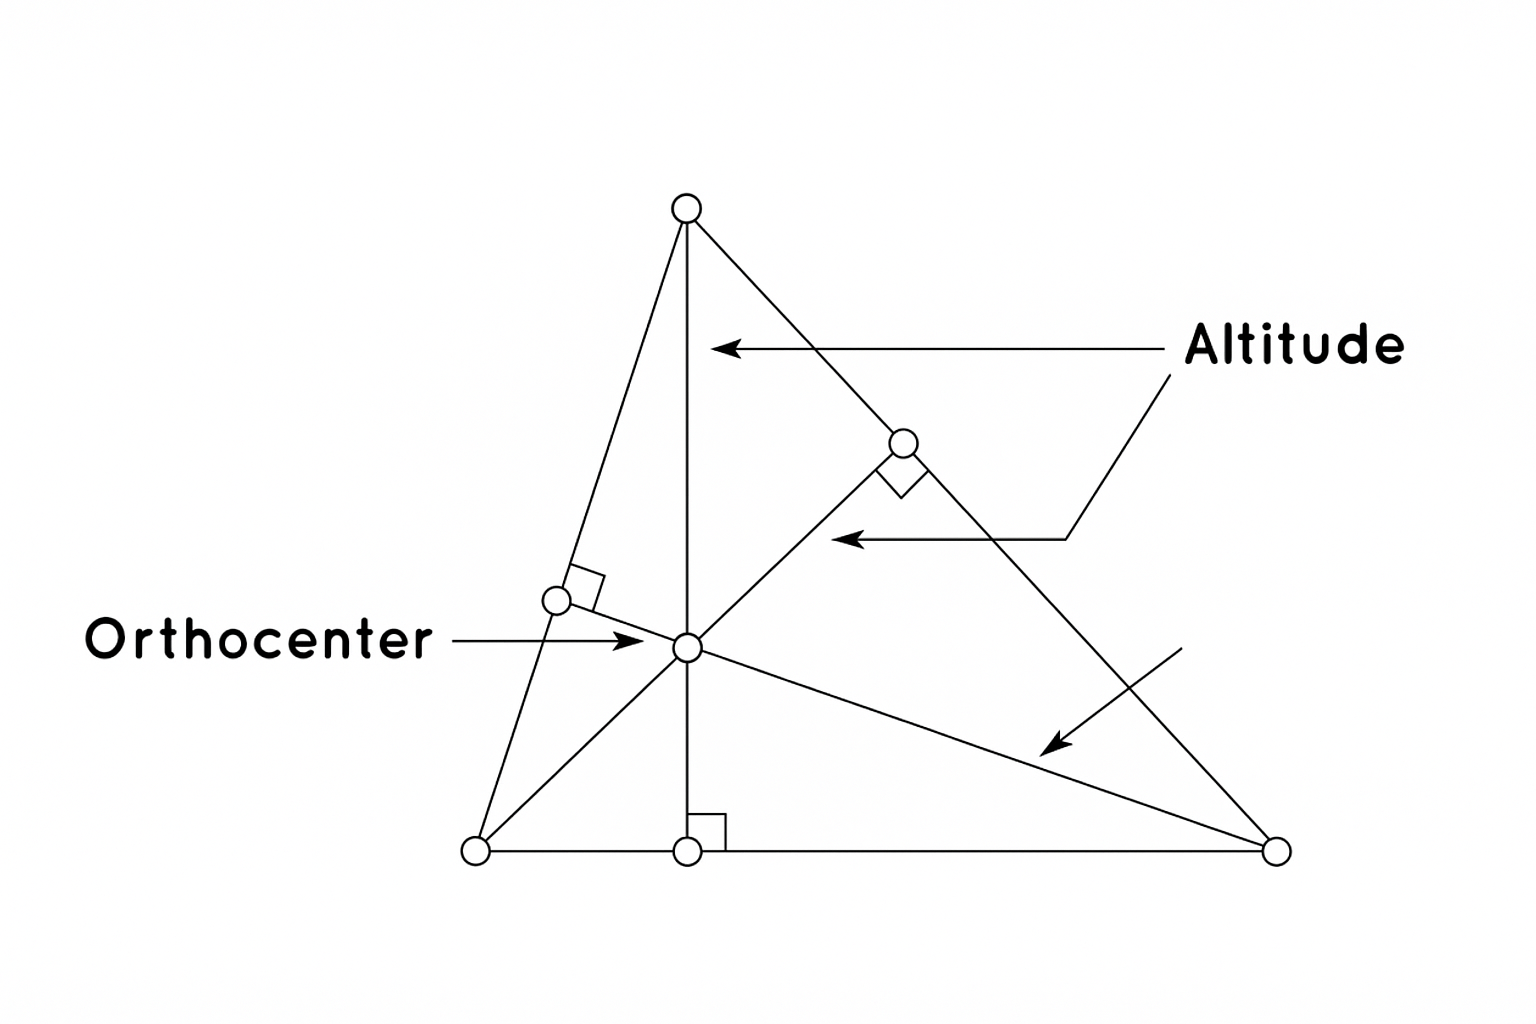
\includegraphics[width=\linewidth]{images/cus06.png}
\end{center}
\begin{choices}
  \choice $\frac{15}{38}$
  \choice $\frac{15}{23}$
  \choice $\frac{23}{15}$
  \CorrectChoice $\frac{38}{15}$
\end{choices}

\question[1]
In $\triangle X Y Z$, the measure of $\angle X$ is $24^{\circ}$ and the measure of $\angle Y$ is $98^{\circ}$. What is the measure of $\angle Z$?
\begin{choices}
  \choice $58^{\circ}$
  \CorrectChoice $58^{\circ}$
  \choice $122^{\circ}$
  \choice $212^{\circ}$
\end{choices}


\newpage

\question[1]
Two nearby trees are perpendicular to the ground, which is flat. One of these trees is 10 feet tall and has a shadow that is 5 feet long. At the same time, the shadow of the other tree is 2 feet long. How tall, in feet, is the other tree?
\begin{choices}
  \CorrectChoice 4
  \choice 3
  \choice 8
  \choice 27
\end{choices}

\question[1]
In the figure, line $m$ is parallel to line $n$. What is the value of $w$?
\begin{center}
  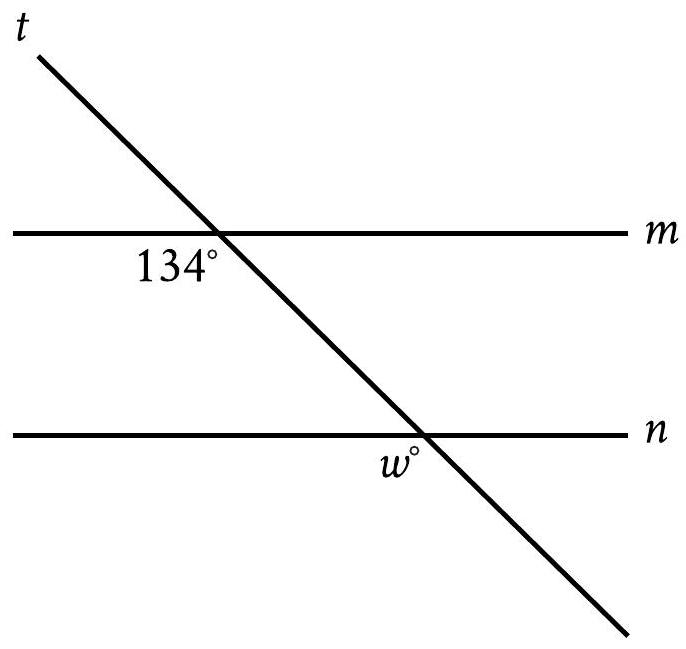
\includegraphics[width=0.90\linewidth]{images/2025_06_15_d0312806c0eedc278ae1g-14}
\end{center}
\begin{choices}
  \choice 13
  \choice 34
  \choice 66
  \choice 134
\end{choices}




\newpage





\question[1]
In triangles $A B C$ and $D E F$, angles $B$ and $E$ each have measure $27^{\circ}$ and angles $C$ and $F$ each have measure $41^{\circ}$. Which additional piece of information is sufficient to determine whether triangle $A B C$ is congruent to triangle $D E F$?
\begin{choices}
  \choice The measure of angle $A$
  \choice The length of side $A B$
  \CorrectChoice The lengths of sides $B C$ and $E F$
  \choice No additional information is necessary
\end{choices}

\question[1]
In triangles $L M N$ and $R S T$, angles $L$ and $R$ each have measure $60^{\circ}, L N=10$, and $R T=30$. Which additional piece of information is sufficient to prove that triangle $L M N$ is similar to triangle $R S T$?
\begin{choices}
  \choice $M N=7$ and $S T=7$
  \choice $M N=7$ and $S T=21$
  \choice The measures of angles $M$ and $S$ are $70^{\circ}$ and $60^{\circ}$, respectively.
  \CorrectChoice The measures of angles $M$ and $T$ are $70^{\circ}$ and $50^{\circ}$, respectively.
\end{choices}


\question[1]
Triangles $A B C$ and $D E F$ are shown above. Which of the following is equal to the ratio $\frac{B C}{A B}$?
\begin{center}
  
\includegraphics[width=0.90\linewidth]{images/cus01.png}
\end{center}
\begin{choices}
  \choice $\frac{D E}{D F}$
  \choice $\frac{D F}{D E}$
  \choice $\frac{D F}{E F}$
  \choice $\frac{E F}{D E}$
\end{choices}



\newpage


\question[1]
In the figure above, what is the length of $\overline{N Q}$?
\begin{center}
  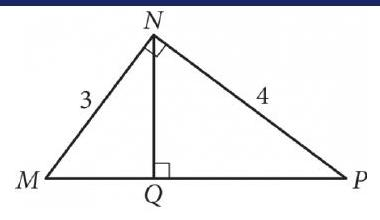
\includegraphics[width=0.90\linewidth]{images/2025_06_15_d0312806c0eedc278ae1g-18}
\end{center}
\begin{choices}
  \choice 2.2
  \choice 2.3
  \choice 2.4
  \choice 2.5
\end{choices}

\question[1]
Triangle $X Y Z$ is similar to triangle $R S T$ such that $X, Y$, and $Z$ correspond to $R, S$, and $T$, respectively. The measure of $\angle Z$ is $20^{\circ}$ and $2 X Y=R S$. What is the measure of $\angle T$?
\begin{choices}
  \choice $2^{\circ}$
  \choice $10^{\circ}$
  \CorrectChoice $20^{\circ}$
  \choice $40^{\circ}$
\end{choices}





\newpage





\question[1]
In the figure shown, lines $r$ and $s$ are parallel, and line $m$ intersects both lines. If $y<65$, which of the following must be true?
\begin{center}
  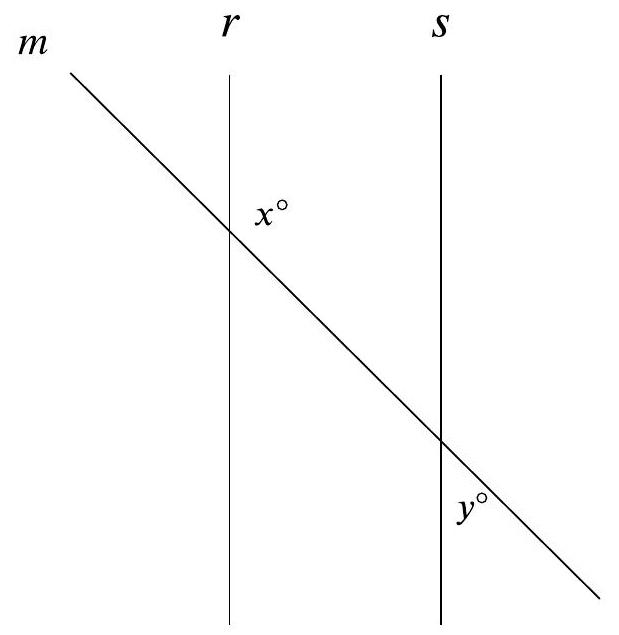
\includegraphics[width=0.90\linewidth]{images/2025_06_15_d0312806c0eedc278ae1g-20}
\end{center}
Note: Figure not drawn to scale.
\begin{choices}
  \choice $x<115$
  \choice $x>115$
  \choice $x+y<180$
  \choice $x+y>180$
\end{choices}


\newpage



\question[1]
In the triangle shown, what is the value of $\sin x^{\circ}$?
\begin{center}
  
\includegraphics[width=0.90\linewidth]{images/cus02.png}
\end{center}

\question[1]
A graphic designer is creating a logo for a company. The logo is shown in the figure above. The logo is in the shape of a trapezoid and consists of three congruent equilateral triangles. If the perimeter of the logo is 20 centimeters, what is the combined area of the shaded regions, in square centimeters, of the logo?
\begin{center}
  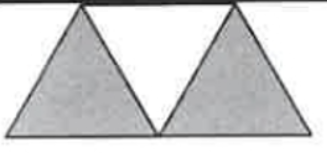
\includegraphics[width=0.90\linewidth]{images/cus03.png}
\end{center}
\begin{choices}
  \choice $2 \sqrt{3}$
  \choice $4 \sqrt{3}$
  \choice $8 \sqrt{3}$
  \choice 16
\end{choices}



\newpage



\question[1]
In the triangle shown, what is the value of $\tan x^{\circ}$?
\begin{center}
  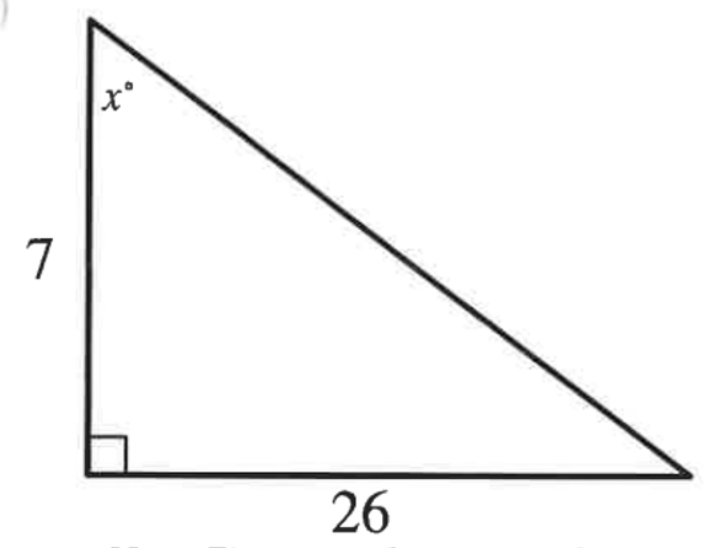
\includegraphics[width=0.90\linewidth]{images/cus04.png}
\end{center}
\begin{choices}
  \choice $\frac{1}{26}$
  \choice $\frac{19}{26}$
  \choice $\frac{26}{7}$
  \choice $\frac{33}{7}$
\end{choices}

\question[1]
The perimeter of an equilateral triangle is 624 centimeters. The height of this triangle is $k \sqrt{3}$ centimeters, where $k$ is a constant. What is the value of $k$?
\begin{solution}
104
\end{solution}



\newpage



\question[1]
In the figure above, $\tan B=\frac{3}{4}$. If $B C=15$ and $D A=4$, what is the length of $\overline{D E}$?
\begin{center}
  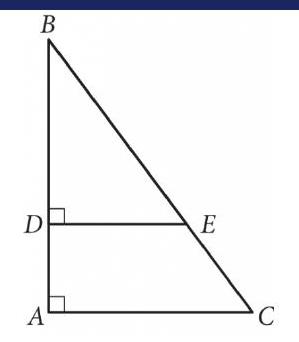
\includegraphics[width=0.90\linewidth]{images/2025_06_15_f612918e7cf8d6fcced3g-10}
\end{center}

\endgradingrange{sat-drill-06}
